\chapter{Solving nonlinear contact examples using element 8-nodes} % Main chapter title

\label{Chapter4 } % For referencing the chapter elsewhere, use \ref{Chapter1} 

%----------------------------------------------------------------------------------------
In this chapter, we consider two examples that are Self-contact example and Rubber Blade
example.After calculating displacement and stress on the model, next we consider the result of
displacement at a specific point on the model and the maximum stress on the contact edge. All the
calculated results from MATLAB will be compared with the results obtained from ANSYS software.
\newpage
\section{Self-contact example}

\subsection{Requirements of the example}

The Figure \ref{fig:contactself_exam} shown the geometry of the Self-contact example.

\begin{figure}[H]
    \centering
    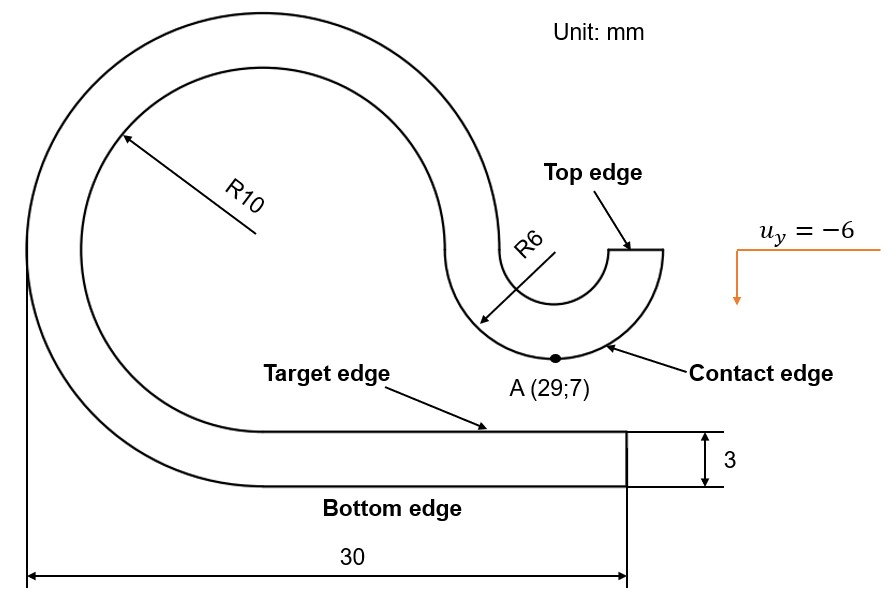
\includegraphics[scale=0.6]{Figures/contactself.jpg}
    \decoRule   
    \caption{Self-contact example}
    \label{fig:contactself_exam}
\end{figure} \noindent
\noindent
The model endures large deformation, when the deformation is large enough the
model will contact itself, technically called Self-contact. The model consists of the circle with
radius 10mm tangent to another circle with radius 6mm; below is Bottom edge which is fixed; above
is the Top edge which is applied displacement is $u_y = - 6 mm$. 
In this example the penalty method is applied to fulfill the contact constraint conditions.
Determine displacement and stress in the model.
Analysing displacement of {\bf point A} and maximal stress in {\bf contact edge} depends on
load step. \\

\newpage
\subsection{Preprocessor}
Element type: 8-nodes (Q8).
\vspace{0.38cm}
\newline
Material props: Neo-hookean model with material properties: the shear modulus ($\mu$) is assumed to 
be $80.194 N/mm^2$ and the bulk modulus ($\kappa$) is $120.291 N/mm^2$.
\vspace{0.38cm} \newline
Frictionless: in this study, contact problems with hyper-elastic materials are
considered in cases of frictionless sliding and frictionless compressing.
\vspace{0.38cm} \newline
Boundary conditions: in this example, we have the following boundary conditions: the Bottom edge is 
constrained displacement in the two directions x, y; Top edge is constrained to displacement in the 
x direction and is applied displacement is $u_y = - 6 mm$.
\vspace{0.38cm} \newline
Mesh: Figure \ref{fig:contactself_mesh_Q8} shown the mesh of the Self-contact example.
There is 357 total number of nodes, and 88 total number of elements.
\begin{figure}[H]
    \centering
    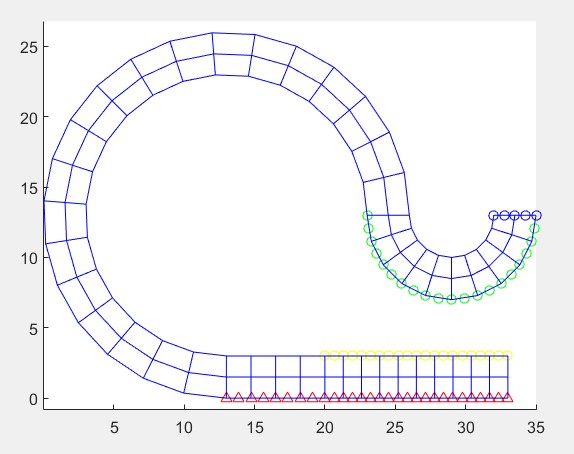
\includegraphics[scale=1]{Figures/contactself_mesh_Q8.jpg}
    \decoRule   
    \caption{Q8 mesh of Contact-self example}
    \label{fig:contactself_mesh_Q8}
\end{figure} \noindent \noindent
Number of steps: 60 steps and the convergence criterion is that of each step the residual force is less than 0.001.
\newpage

\subsection{Displacement}
\begin{figure}[H]
    \centering
    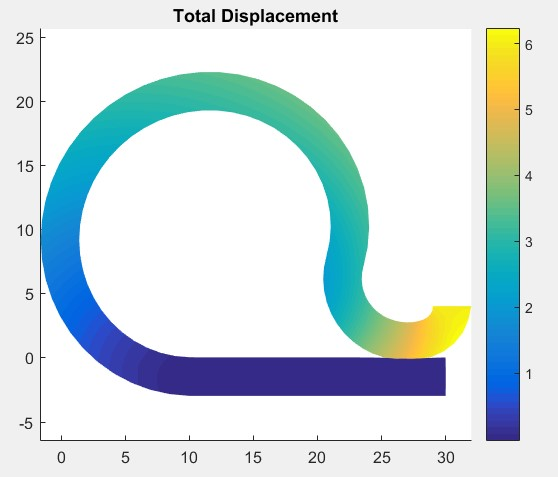
\includegraphics[scale=0.6]{Figures/t_displace_self_q8_matlab.jpg}
    \decoRule
    \caption{Total displacement of Contact-self example \\ (Q8 MATLAB)}
    \label{fig:t_displace_self_q8_matlab}
\end{figure} \noindent

\begin{figure}[H]
    \centering
    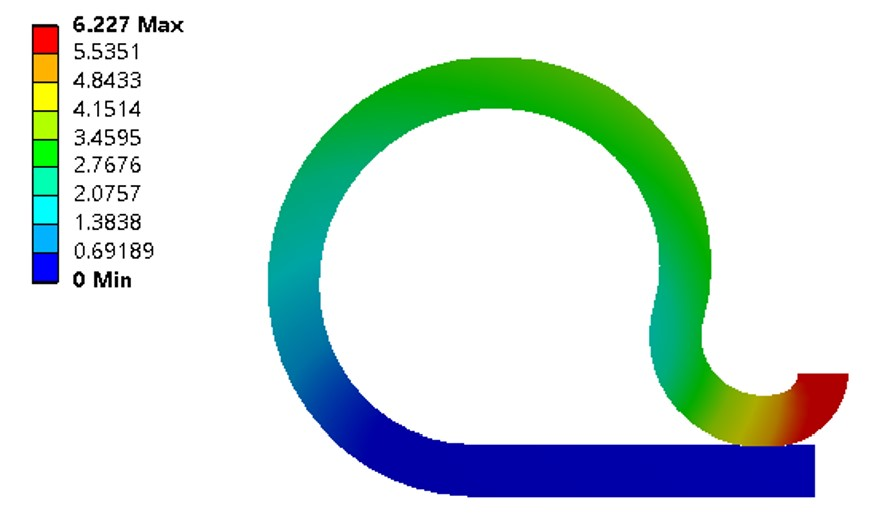
\includegraphics[scale=0.5]{Figures/t_displace_self_q8_ansys.jpg}
    \decoRule   
    \caption{Total displacement of Contact-self example \\ (Q8 ANSYS)}
    \label{fig:t_displace_self_q8_ansys}
\end{figure} \noindent
The total displacement is shown in the Figure \ref{fig:t_displace_self_q8_matlab}.
The Top edge is applied a vertical displacement -6 mm, so the contact edge is pressed down to the target edge. Because of the frictionless, the contact edge is not subsidence at the area where is contact with the target edge.
Then, the contact edge is sliced to the left side.
\vspace{0.38cm} \newline
The comparison of the total displacement between this study result and the reference result
is shown in the Figure \ref{fig:t_displace_self_q8_matlab} and Figure \ref{fig:t_displace_self_q8_ansys}.
So, there have not large difference between them.
The error of maximum total displacement between MATLAB solution and ANSYS solution is $0.1\%$
\newpage 
\noindent
To compare carefully, point A are considered in horizontal and vertical displacement. 
Figure \ref{fig:xA_displace_self_q8_matlab} shown the horizontal displacement of point A. 
Figure \ref{fig:yA_displace_self_q8_matlab} shown the vertical displacement of point A.
\vspace{0.38cm}
\begin{figure}[H]
    \centering
    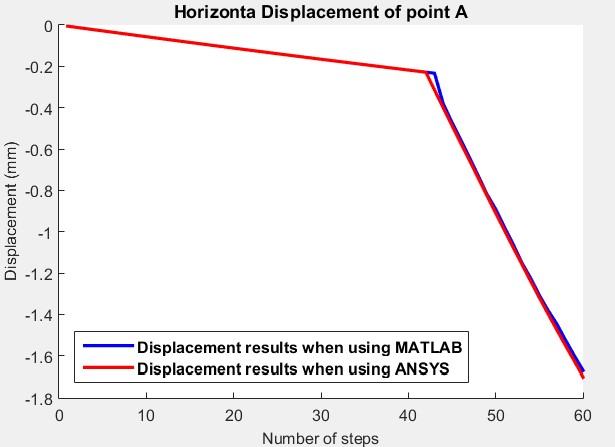
\includegraphics[scale=0.72]{Figures/xA_displace_self_q8_matlab.jpg}
    \decoRule
    \caption{Horizontal displacement of point A}
    \label{fig:xA_displace_self_q8_matlab}
\end{figure} \noindent.
\begin{figure}[H]
    \centering
    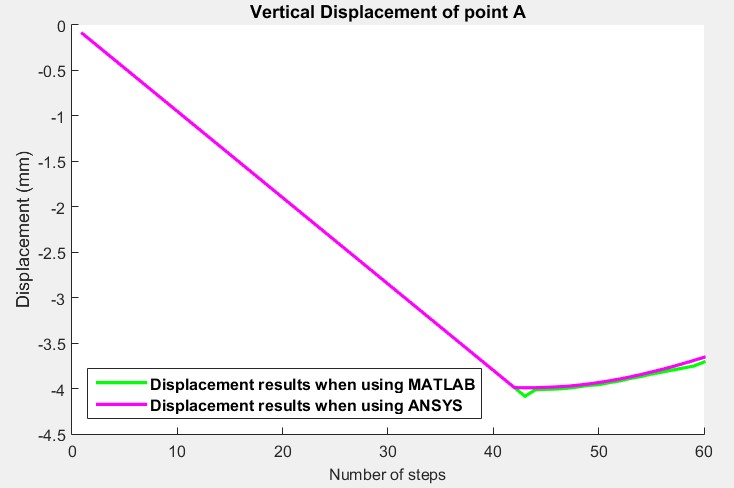
\includegraphics[scale=0.6]{Figures/yA_displace_self_q8_matlab.jpg}
    \decoRule
    \caption{Vertical displacement of point A}
    \label{fig:yA_displace_self_q8_matlab}
\end{figure} \noindent
At the point A, the displacement have a bit variability in load step 42.
Because here point A starts to touch the Target edge and 
there is a difference between how the problem is solved in the MATLAB program 
and in the ANSYS software.
\vspace{0.38cm} \newline
Follow Figure \ref{fig:xA_displace_self_q8_matlab}, we can see that 
the horizontal displacement of point A increases slowly before load step 42.
Before this load step, point A has not slipped on the Target edge.
After load step 42, point A slips on Target edge so horizontal displacement increases faster
\vspace{0.38cm} \newline
Follow Figure \ref{fig:yA_displace_self_q8_matlab}, we can see that
the vertical displacement of point A increases rapidly before load step 42,
then point A tends to go up.
Before this load step, point A has not slipped on the Target edge 
which means that point A is not obstructed in the vertical direction
After load step 42, point A slips on Target edge so point A can't go through the Target edge.
\subsection{Stress distribution}
\begin{figure}[H]
    \centering
    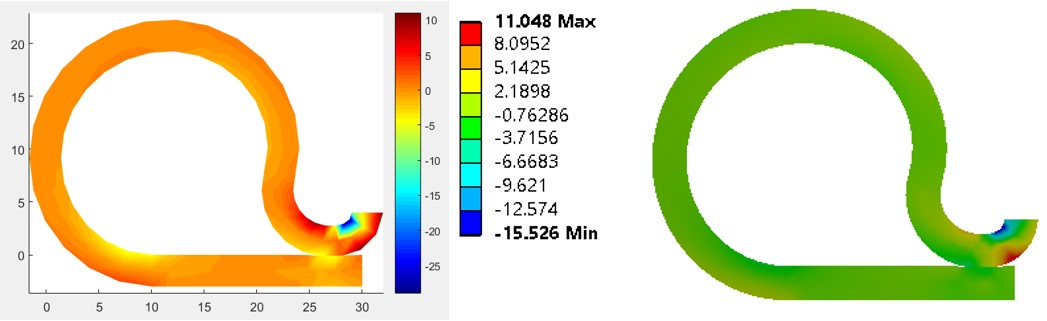
\includegraphics[scale=0.55]{Figures/sx_self_MandA.jpg}
    \decoRule
    \caption{Normal stress $\sigma_x$ of Contact-self example \\(MATLAB results on the left, ANSYS results on the right)}
    \label{fig:sx_self_MandA}
\end{figure} \noindent
Figure \ref{fig:sx_self_MandA} shown the normal stress $\sigma_x$ contour plot of the Contact-self example,
the left figure shown the contour plot of this study and the right one is the result of
commercial program (ANSYS). There are many stress concentration areas (compressive
stress and tensile stress), this figure also shown the comparison of the normal stress $\sigma_x$
distributions, it shown that the stress distributions are similar, 
so the normal stress $\sigma_x$ results can be acceptable.
Error of maximum normal stress $\sigma_x$ between MATLAB results and ANSYS is $1.13\%$
\\
\begin{figure}[H]
    \centering
    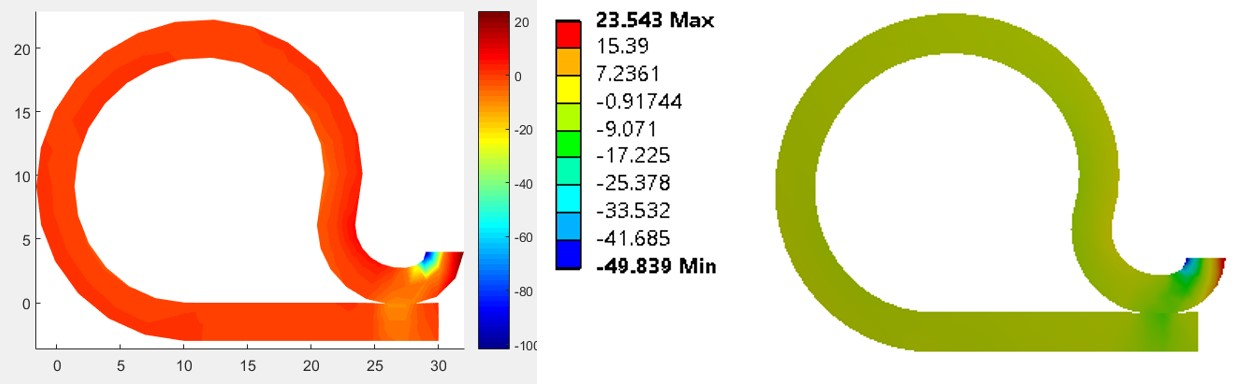
\includegraphics[scale=0.5]{Figures/sy_self_MandA.jpg}
    \decoRule
    \caption{Normal stress $\sigma_y$ of Contact-self example \\(MATLAB results on the left, ANSYS results on the right)}
    \label{fig:sy_self_MandA}
\end{figure} \noindent
Figure \ref{fig:sy_self_MandA} shown the normal stress $\sigma_y$ contour plot of the Contact-self example, 
the left figure shown the contour plot of this study and the right one is the result of commercial
program (ANSYS). Like Figure \ref{fig:sx_self_MandA},
from the results in the Figure \ref{fig:sy_self_MandA} there are many stress concentration areas (compressive and tensile stress),
it also shows a comparison of the normal stress $\sigma_y$ distributions,
showing that the stress distribution is similar,
since the result of normal stress $\sigma_y$ results is acceptable.
Error of maximum normal stress $\sigma_y$ between MATLAB results and ANSYS is $0.18\%$
\vspace{0.38cm} \newline
To specifically compare the variation of normal stress between MATLAB program and ANSYS software,
we consider the stress on contact edge under load strep.
Maximum stress in the contact edge is said to be an important component in the contact problem,
if the stress exceeds the allowable limit,
it is possible that on the contact edge, the model will be damaged.
\vspace{0.38cm} \newline
Maximum normal stress $\sigma_x$ and $\sigma_y$ of the contact edge will show in
Figure \ref{fig:sx_self_contact} and Figure \ref{fig:sy_self_contact}
\vspace{0.38cm}
\begin{figure}[H]
    \centering
    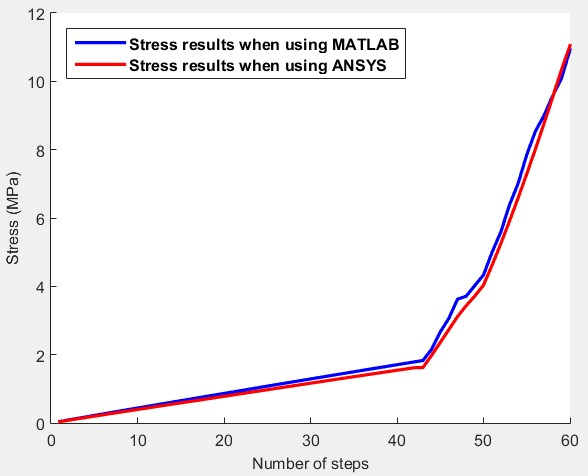
\includegraphics[scale=0.55]{Figures/sx_self_contact.jpg}
    \decoRule
    \caption{Normal stress $\sigma_x$ of contact edge}
    \label{fig:sx_self_contact}
\end{figure} \noindent

\begin{figure}[H]
    \centering
    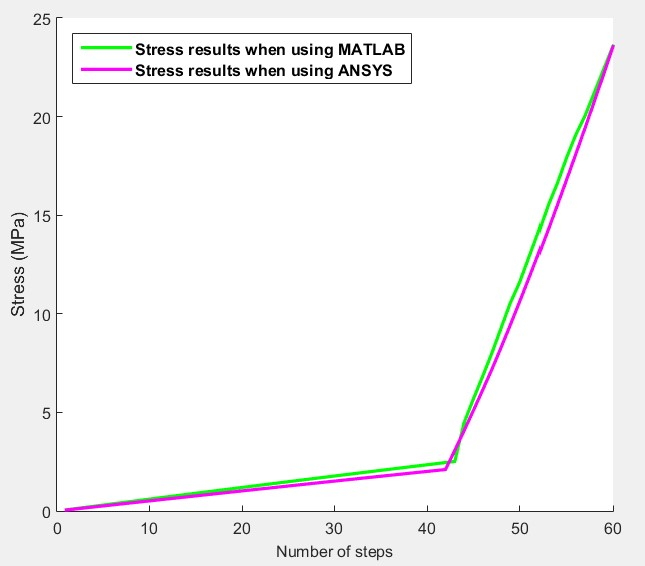
\includegraphics[scale=0.5]{Figures/sy_self_contact.jpg}
    \decoRule
    \caption{Normal stress $\sigma_y$ of contact edge}
    \label{fig:sy_self_contact}
\end{figure} \noindent
Look at Figure \ref{fig:sx_self_contact} and Figure \ref{fig:sy_self_contact},
we can see that the result of stress according to the load step 
between MATLAB results and ANSYS results is quite similar. Maximum normal stress $\sigma_x$ and maximum normal stress $\sigma_y$ both increase slowly before load step 42.
Since before this load step the Contact edge has not been in contact with the Target edge, the stress generated is mainly due to the deformation of the material.
After load step 42, the Contact edge contacts and slides on the Target edge; rapid increase in stress; In this stage, the stress generated is mainly due to the contact force between the upper part and the lower part.
Due to applied displacement in the y direction, the stress in the y direction is predominant and significantly larger than the stress in the x direction. 
\section{Rubber Blade example}
\subsection{Requirements of the example}
The Figure \ref{fig:model_rubber} shown the geometry of the Rubber Blade example
\begin{figure}[H]
    \centering
    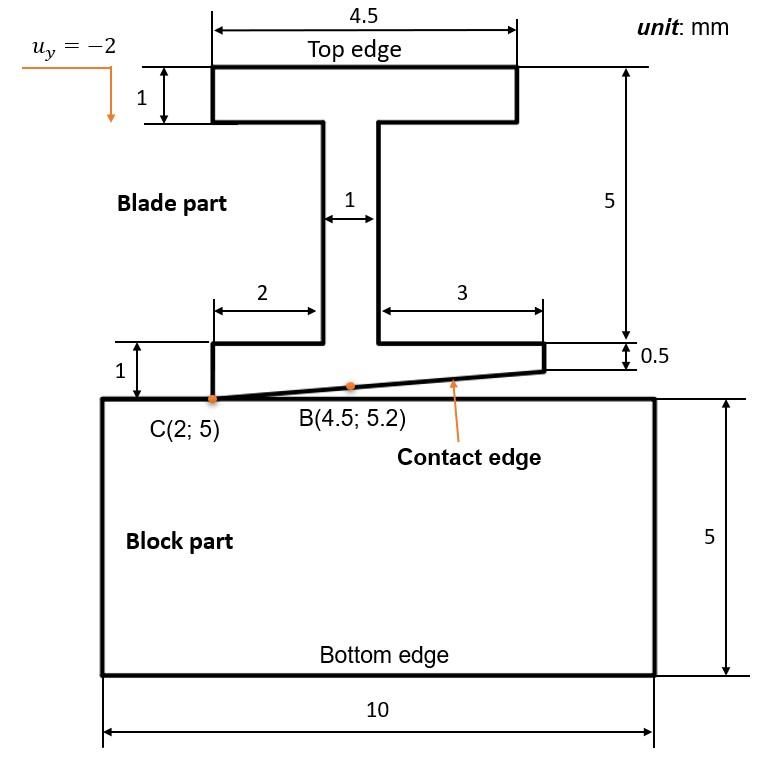
\includegraphics[scale=0.75]{Figures/model_rubber.jpg}
    \decoRule
    \caption{Rubber Blade example}
    \label{fig:model_rubber}
\end{figure}
\noindent
Different from Self-contact example, in this case, large sliding of the cross section of an elastic rubber blade is considered.
The rubber blade is subjected to a vertical prescribed displacement and pressed against a rubber block.
The contact is assumed to be frictionless.
In this example the penalty method is applied to fulfill the contact constraint conditions.
Determine displacement and stress in the model.
Analysing displacement of {\bf point B}, {\bf point C} and maximal stress in {\bf Contact edge} depends on load step.
\newpage
\subsection{Preprocessor}
Element type: 8-nodes (Q8).
\vspace{0.38cm} \newline
Material props: Neo-hookean model with material properties: the shear modulus ($\mu$) is assumed to 
be $80.194 N/mm^2$ and the bulk modulus ($\kappa$) is $60.291 N/mm^2$.
\vspace{0.38cm} \newline
Frictionless: in this study, contact problems with hyper-elastic materials are
considered in cases of frictionless sliding and frictionless compressing.
\vspace{0.38cm} \newline
Boundary conditions:
There is a vertical displacement applied in the top edge of the rubber blade. 
In this example, the vertical displacement is 2 mm. The contact areas are the bot edge of the rubber blade and the top edge of the block.
The block is fixed at the bottom.
\vspace{0.38cm} \newline
Mesh: Figure \ref{fig:mesh_rub} shown the mesh of the Self-contact example.
There is 435 total number of nodes, and 113 total number of elements.
\begin{figure}[H]
    \centering
    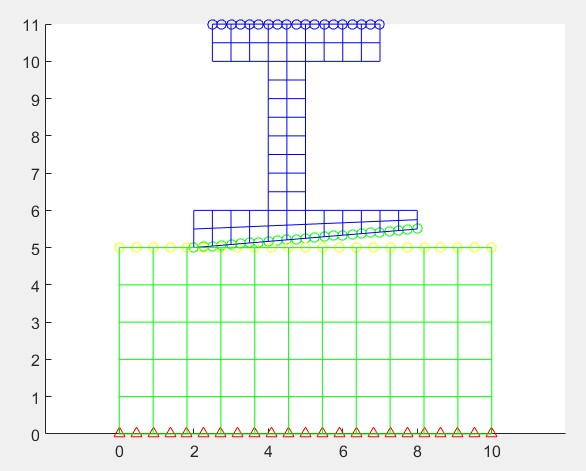
\includegraphics[scale=1]{Figures/mesh_rub.jpg}
    \decoRule
    \caption{Q8 mesh of Rubber Blade example}
    \label{fig:mesh_rub}
\end{figure} \noindent
Number of steps: 20 steps and the convergence criterion is that of each step the residual force is less than 0.001.
\newpage
\subsection{Displacement}
\begin{figure}[H]
    \centering
    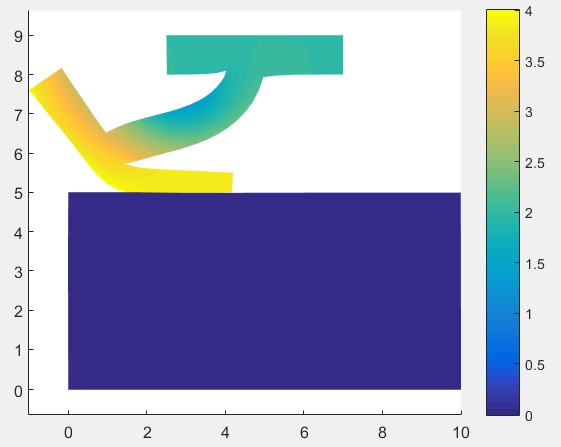
\includegraphics[scale=0.8]{Figures/dt_rub_mat.jpg}
    \decoRule
    \caption{Total displacement of rubber blade example (MATLAB)}
    \label{fig:dt_rub_mat}
\end{figure} \noindent
\begin{figure}[H]
    \centering
    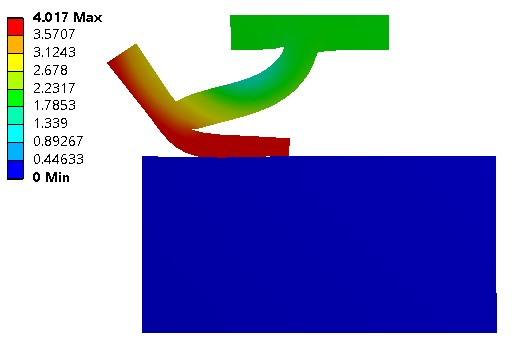
\includegraphics[scale=1]{Figures/dt_rub_an.jpg}
    \decoRule
    \caption{Total displacement of rubber blade example (ANSYS)}
    \label{fig:dt_rub_an}
\end{figure} \noindent
The total displacement is shown in the Figure \ref{fig:dt_rub_mat}. The blade is applied a vertical
displacement 2 mm, so the blade is pressed down to the block. Because of the frictionless,
the block is not subsidence at the area where is contact with the blade. Then, the bottom
side of the blade is sliced to the left side.
\vspace{0.38cm} \newline
The comparison of the total displacement between this study result and the reference result
is shown in the Figure \ref{fig:dt_rub_mat} and Figure \ref{fig:dt_rub_an}. So, there have not large difference between them. 
The error of maximum total displacement between MATLAB solution and ANSYS solution is $0.3\%$.
\vspace{0.38cm} \newline
To compare carefully, two points (B and C) are considered in vertical and horizontal displacement during load steps.
Figure \ref{fig:disB} shown the displacement of point B, and Figure \ref{fig:dc}  shown the displacement of point C.
\begin{figure}[H]
    \centering
    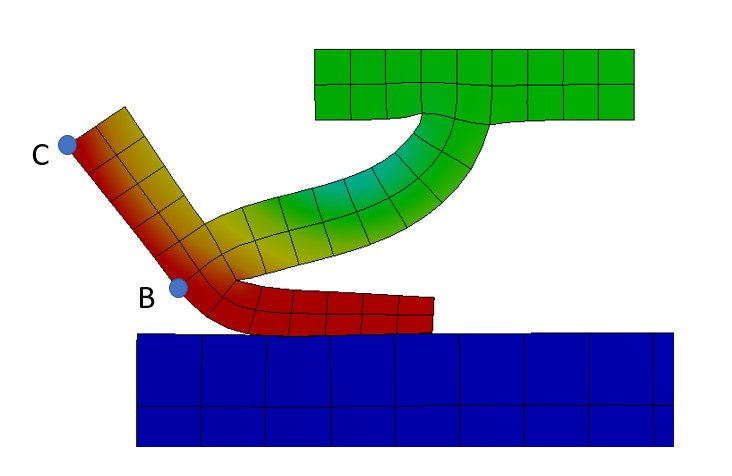
\includegraphics[scale=0.75]{Figures/dbdc.jpg}
    \decoRule
    \caption{Position of point B and C}
    \label{fig:dbdc}
\end{figure} \noindent
\begin{figure}[H]
    \centering
    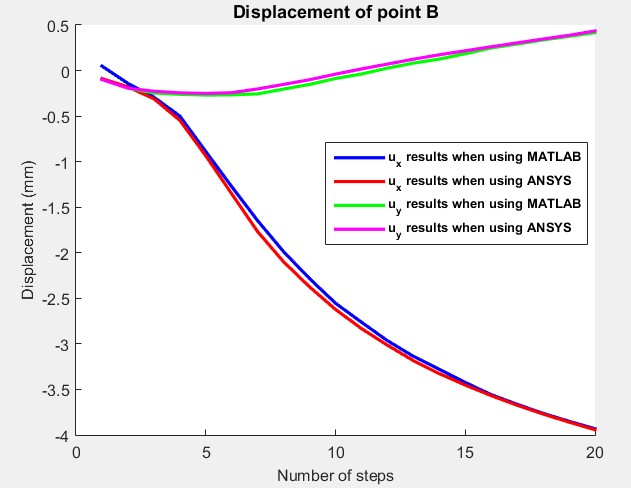
\includegraphics[scale=0.8]{Figures/disB.jpg}
    \decoRule
    \caption{Displacement of point B}
    \label{fig:disB}
\end{figure} \noindent
At the point B, the vertical displacement have a bit variability, because of the nonlinear
behavior of contact, at the beginning, the point A have to be moved a small distance (0 to
5 load step) to contact with the block.  After that, the point A moved up because the
contact reaction forces. Also after sliding on block part, contact edge tends to go up.
For the horizontal displacement, there is the rapid rise of the
displacement in load step 0 to 5, because point A has not been in contact with {\bf the block part}, then point A slides to the left at this time the horizontal displacement of point A increases rapidly.
\newline
\begin{figure}[H]
    \centering
    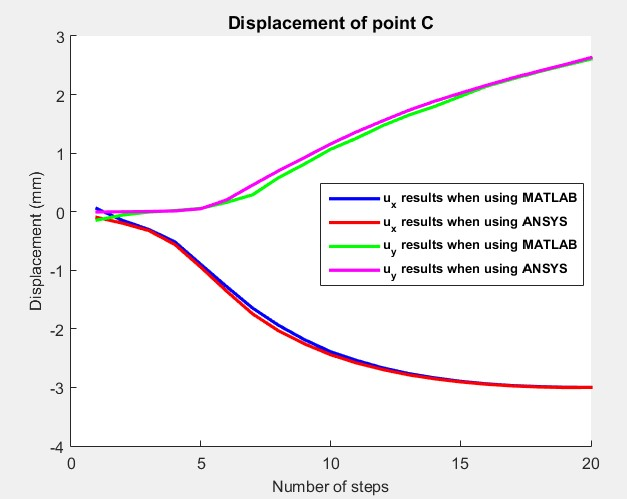
\includegraphics[scale=0.83]{Figures/dc.jpg}
    \decoRule
    \caption{Displacement of point B}
    \label{fig:dc}
\end{figure} \noindent
For the point C, the vertical displacement is almost the same as the point B, but there is no downward displacement stage. Vertical displacement slows up in the early stages, where point C just slipped off the block part. 
After about 7th load step, point C tends to go up due to the general deformation of the model.
For the horizontal displacement, there is a stage (load step 0 to 5) which increases slowly. Because in this stage the contact edge begins to approach the block part, the slip has not taken place much, so point C has a little horizontal displacement.
After 7th load step, contact edge completely slides on the block part, the slip has taken place much, point C moves left faster.
\newpage
\subsection{Stress distribution}
\begin{figure}[H]
    \centering
    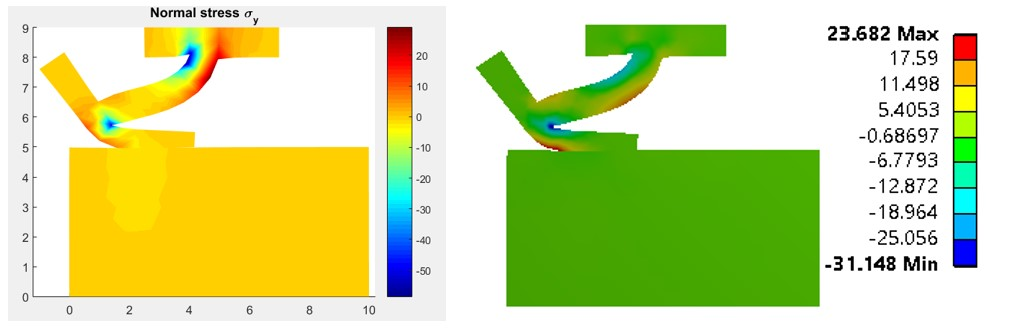
\includegraphics[scale=0.63]{Figures/sx_rub_MvsA.jpg}
    \decoRule
    \caption{Normal stress $\sigma_x$ of rubber blade example \\(MATLAB results on the left, ANSYS results on the right)}
    \label{fig:sx_rub_MvsA}
\end{figure} \noindent
Figure \ref{fig:sx_rub_MvsA} shown the normal stress $\sigma_x$ contour plot of the rubber blade example,
the left figure shown the contour plot of this study and the right one is the result of
commercial program (ANSYS). There are many stress concentration areas (compressive
stress and tensile stress), this figure also shown the comparison of the normal stress $\sigma_x$
distributions, it shown that the stress distributions are similar, so the normal
stress $\sigma_x$ results can be acceptable.
Error of maximum normal stress $\sigma_x$ between MATLAB results and ANSYS is $0.85\%$.
\newline
\begin{figure}[H]
    \centering
    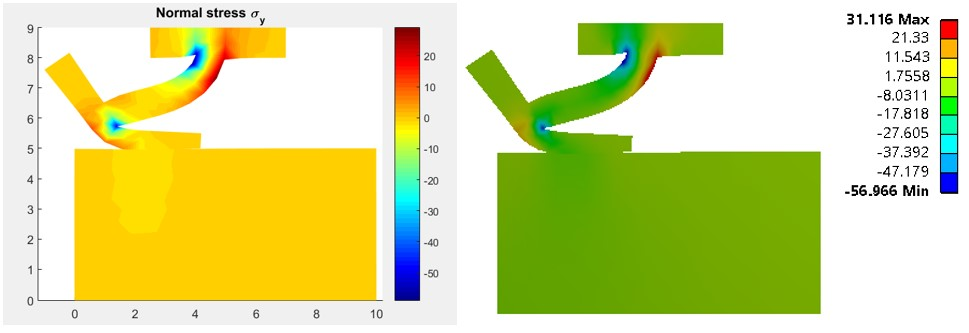
\includegraphics[scale=0.65]{Figures/sy_rub_MvsA.jpg}
    \decoRule
    \caption{Normal stress $\sigma_y$ of rubber blade example \\(MATLAB results on the left, ANSYS results on the right)}
    \label{fig:sy_rub_MvsA}
\end{figure} \noindent
\noindent
Figure \ref{fig:sy_rub_MvsA} shown the normal stress $\sigma_y$ contour plot of the rubber blade example, the
left figure shown the contour plot of this study and the right one is the result of commercial
program (ANSYS). Like Figure 4.6, there are also many stress concentration areas (compressive
stress and tensile stress). It shown that the stress distributions are similar, so the normal $\sigma_y$
stress results can be acceptable.
Error of maximum normal stress $\sigma_y$ between MATLAB results and ANSYS is $6.85\%$.
We can see that the error of maximum normal stress $\sigma_y$ is significant (greater than $5\%$).
It's very likely due to applied displacement is $u_y = - 2 mm$ in top edge leads to compression in the y-direction, the error is mainly in the y-direction.
\vspace{0.38cm}
\newline 
Different from self-contact example, rubber blade example has a larger normal stress error.
This is understandable as the rubber blade example model is more complex than the self-contact example model. The model has more stress concentrations areas (shown in Figure \ref{fig:s_tt}).
In addition, the contact area of the rubber blade example (line to line) is larger than the contact area of the self-contact example (nearly node to line).
Self-contact example model we have only one part and rubber blade example model we have tow parts that are in contact with each other.
Furthermore, we are using 8 node element, it is suitable for problems with curves model.
\begin{figure}[H]
    \centering
    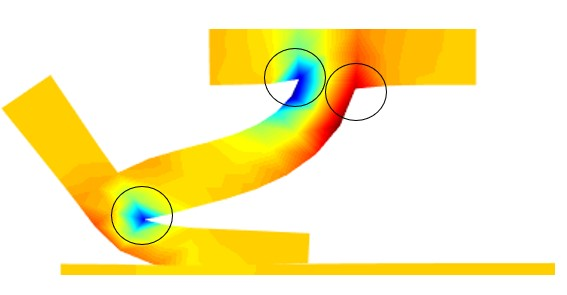
\includegraphics[scale=0.7]{Figures/s_tt.jpg}
    \decoRule
    \caption{Stress concentrations areas of rubber blade example}
    \label{fig:s_tt}
\end{figure} \noindent
To specifically compare the variation of normal stress between MATLAB program and ANSYS software,
we consider the stress on contact edge during load strep.
Maximum stress in the contact edge is said to be an important component in the contact problem,
if the stress exceeds the allowable limit,
it is possible that on the contact edge, the model will be damaged.
\vspace{0.38cm} \newline
Maximum normal stress $\sigma_x$ and $\sigma_y$ of the contact edge will show in
Figure \ref{fig:sx_c_r} and Figure \ref{fig:sy_c_r}
\newline
\begin{figure}[H]
    \centering
    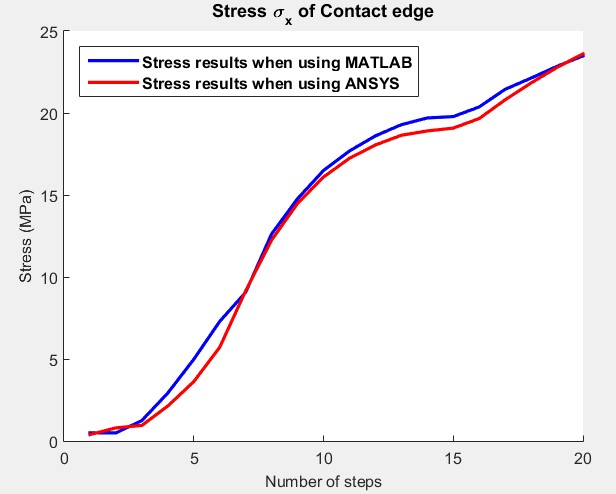
\includegraphics[scale=0.7]{Figures/sx_c_r.jpg}
    \decoRule
    \caption{Normal stress $\sigma_x$ of the contact edge}
    \label{fig:sx_c_r}
\end{figure} \noindent
Figure \ref{fig:sx_c_r} shown the comparison of the normal stress $\sigma_x$ in the contact edge during load step.
The shapes of twos curve are similar, but the values in many load step are different.
The reasons of this error are mesh quality, nonlinear behavior of large deformation and material and that may also be due to the difference between MATLAB and ANSYS solutions.
\vspace{0.38cm}
\begin{figure}[H]
    \centering
    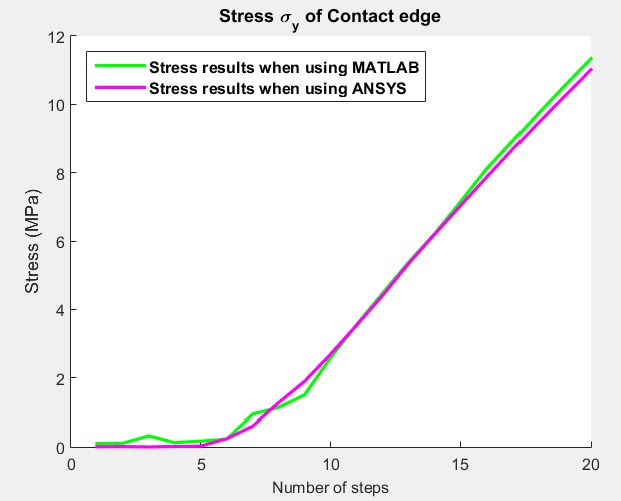
\includegraphics[scale=0.7]{Figures/sy_c_r.jpg}
    \decoRule
    \caption{Normal stress $\sigma_y$ of the contact edge}
    \label{fig:sy_c_r}
\end{figure} \noindent
Figure \ref{fig:sx_c_r} shown the comparison of the normal stress $\sigma_y$ in the contact edge during load step. Normal stress $\sigma_y$ increases rapidly after the 7th load step because the contact edge has made full contact with the block part.
The shapes of twos curve are similar, but the values in many load step are different. Same as normal stress $\sigma_x$,
the reasons of this error are mesh quality, nonlinear behavior of large deformation and material and that may also be due to the difference between MATLAB and ANSYS solutions.
\newline
\section{Discussion}
After solving two example problems, we can confirm that it is possible to apply the 8-nodes element to computational programming. With the computer increasingly upgraded in both hardware and software, the problem of the long solving time of the 8-nodes element has been overcome.
\vspace{0.38cm}
\newline
By solving the self-contact example, we can see that the 8-nodes element gives little error for the model with many curves.
The high order approximation for the finite element {\bf (keeping the same size)} leads to the small error for the solution.